\documentclass[11pt]{article}

\usepackage[margin=1in]{geometry}
\usepackage{booktabs}
\usepackage{amsmath}
\usepackage{tikz}
\usetikzlibrary{positioning,arrows.meta}
\usepackage{caption}
\usepackage{enumitem}

\tikzset{
  io/.style={draw, rounded corners=2pt, align=center, inner sep=5pt,
             minimum width=7.2cm, font=\small},
  stage/.style={draw, align=center, inner sep=5pt,
               minimum width=7.2cm, font=\small},
  diff/.style={draw, align=center, inner sep=5pt,
               minimum width=7.2cm, font=\small, fill=gray!12},
  arr/.style={-{Stealth[length=2.2mm]}, thick}
}

\newcommand{\probehdr}{%
  \toprule
  Fact & Embed & Block 1 & Block 2 & Block 3 & Block 4 \\
  \midrule
}

\title{What the probes read\\in the five Coulomb networks}
\author{Achuthan Rathinam}
\date{8 October 2026}

\begin{document}
\maketitle

\section{What a minus means}

Two different scores appear in the tables, and a minus means a different thing for each.

\paragraph{Probe score, written as $R^2$.}
The probe is a straight line fitted on the training systems and scored on the 4{,}000 validation systems.
\[
R^2 = 1 - \frac{\text{squared error of the line}}{\text{squared error of guessing the validation average}}.
\]
A score of $1$ means the line reads the fact perfectly.
A score of $0$ means the line is no better than guessing the average value of that fact.
A \textbf{negative} score means the line is worse than that guess.
The training fit did not carry over, and its predictions on new systems are actively far from the labels.
It does not mean the physical quantity itself is negative.
The large entry $-2.344$ for potential energy in block~4 of the non-equivariant network is this kind of failure: the line misses by much more than the average would have.

\paragraph{Arrow score, written as cosine.}
Force direction is not an $R^2$.
For each pair the model's own edge update is compared with the true Coulomb force:
\[
\cos\theta = \frac{\text{update}\cdot\text{force}}{|\text{update}|\,|\text{force}|}.
\]
The table reports the average of that cosine over pairs.
$+1$ means the update points the same way as the force.
$0$ means the two arrows are unrelated.
A \textbf{negative} cosine means the update points opposite the true force.
$-1$ would be exactly backward.
The shifted column in the raw logs is the same cosine after the forces are paired with the wrong system.
A real alignment has to sit well above that shifted number.

\section{What every network is given}

None of the probed facts except the charges and the positions are handed to the network.
Charge product, force magnitude, force direction, and potential energy are computed afterwards from the simulator, and the probe tries to read them back out.

\begin{table}[ht]
\centering
\caption{Inputs of one system of 10 particles.
The edge table is not a force matrix.
A 1 means the pair is allowed to interact.
The diagonal is 0, so a particle does not interact with itself.}
\label{tab:inputs}
\begin{tabular}{lll}
\toprule
Array & Shape & Contents \\
\midrule
Charge one-hot & $10 \times 2$ & $[1,0]$ if charge $-1$, $[0,1]$ if charge $+1$ \\
Position & $10 \times 3$ & starting $x,y,z$ \\
Velocity & $10 \times 3$ & starting velocity \\
Edges & $10 \times 10$ & 1 for every pair, 0 on the diagonal \\
\bottomrule
\end{tabular}
\end{table}

The training target is the position of each particle after 1{,}000 simulator steps.
The loss is the mean squared error between those positions and the network's guess.
Lower is better.
The graph layers calculate squared distance themselves by subtracting the two positions.
They do not receive a distance matrix, a force matrix, or the potential energy.

\section{The five architectures}

The three message-passing networks share one block.
The drawings that follow mark the single change that makes each variant.
In all three, and in the equivariant transformer, the positions themselves are not moved inside the block.
The block adds a learned push into the velocity, and the guess is
\[
\text{predicted position} = \text{initial position} + \text{updated velocity}.
\]
That is one shot.
It is not a replay of the 1{,}000 simulator steps.
Widths below are the full models that produced the later tables: hidden width 64, message width 32, four blocks, except where a network is different.

\begin{figure}[ht]
\centering
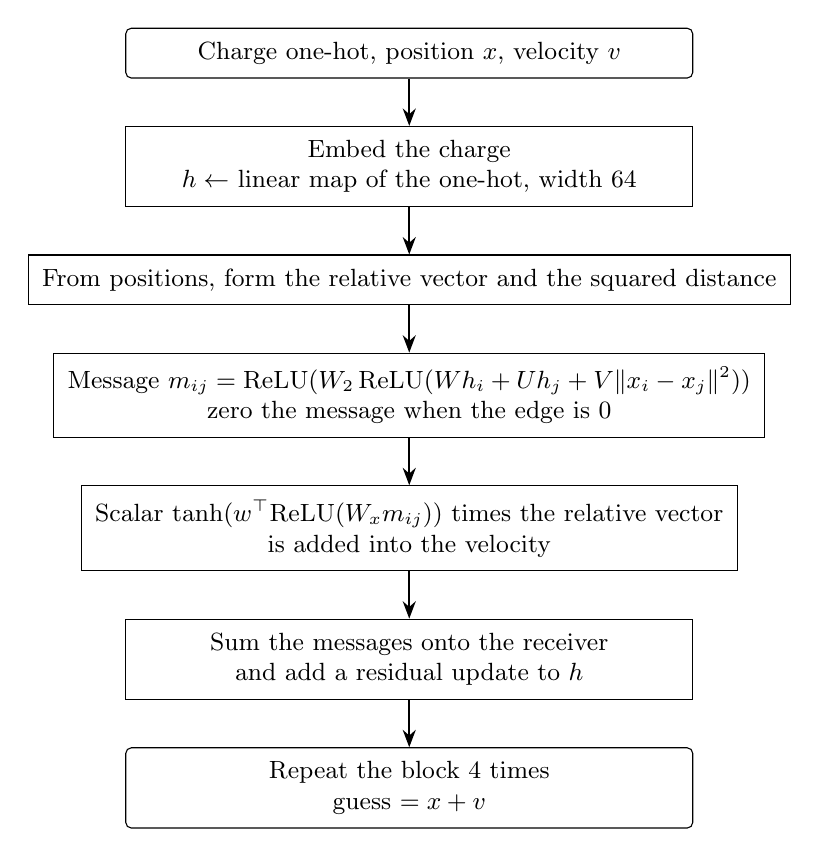
\begin{tikzpicture}
  \node[io] (in) {Charge one-hot, position $x$, velocity $v$};
  \node[stage, below=6mm of in] (emb) {Embed the charge\\$h \leftarrow$ linear map of the one-hot, width 64};
  \node[stage, below=6mm of emb] (dist) {From positions, form the relative vector and the squared distance};
  \node[stage, below=6mm of dist] (msg) {Message $m_{ij} = \mathrm{ReLU}(W_2\,\mathrm{ReLU}(W h_i + U h_j + V\|x_i-x_j\|^2))$\\zero the message when the edge is 0};
  \node[stage, below=6mm of msg] (vel) {Scalar $\tanh(w^\top \mathrm{ReLU}(W_x m_{ij}))$ times the relative vector\\is added into the velocity};
  \node[stage, below=6mm of vel] (hup) {Sum the messages onto the receiver\\and add a residual update to $h$};
  \node[io, below=6mm of hup] (out) {Repeat the block 4 times\\guess $= x + v$};
  \draw[arr] (in) -- (emb);
  \draw[arr] (emb) -- (dist);
  \draw[arr] (dist) -- (msg);
  \draw[arr] (msg) -- (vel);
  \draw[arr] (vel) -- (hup);
  \draw[arr] (hup) -- (out);
\end{tikzpicture}
\caption{EGNN.
The block is the Assignment~2 baseline.
Distance enters only as a squared length, so the message is unchanged by a rotation of the whole system.}
\label{fig:egnn}
\end{figure}

\begin{figure}[ht]
\centering
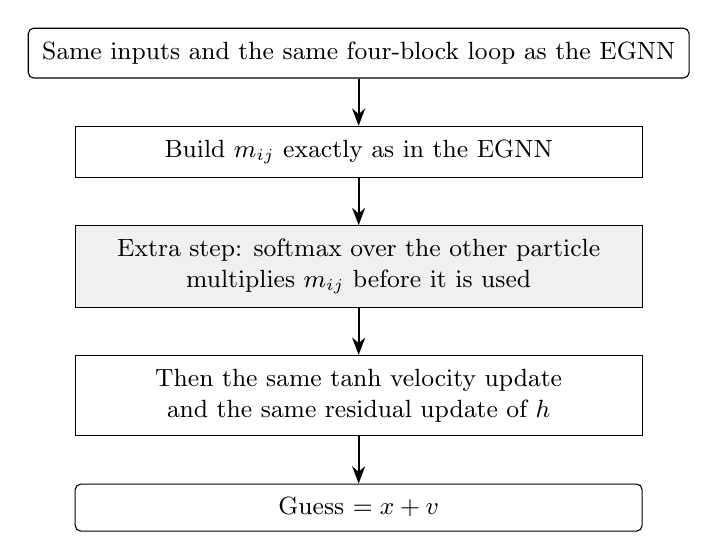
\begin{tikzpicture}
  \node[io] (in) {Same inputs and the same four-block loop as the EGNN};
  \node[stage, below=6mm of in] (msg) {Build $m_{ij}$ exactly as in the EGNN};
  \node[diff, below=6mm of msg] (attn) {Extra step: softmax over the other particle\\multiplies $m_{ij}$ before it is used};
  \node[stage, below=6mm of attn] (rest) {Then the same tanh velocity update\\and the same residual update of $h$};
  \node[io, below=6mm of rest] (out) {Guess $= x + v$};
  \draw[arr] (in) -- (msg);
  \draw[arr] (msg) -- (attn);
  \draw[arr] (attn) -- (rest);
  \draw[arr] (rest) -- (out);
\end{tikzpicture}
\caption{Attention EGNN.
The shaded box is the only change.
The attention weight depends on the message, which depends on charges and distance, so a rotation still does not change the message.}
\label{fig:attn}
\end{figure}

\begin{figure}[ht]
\centering
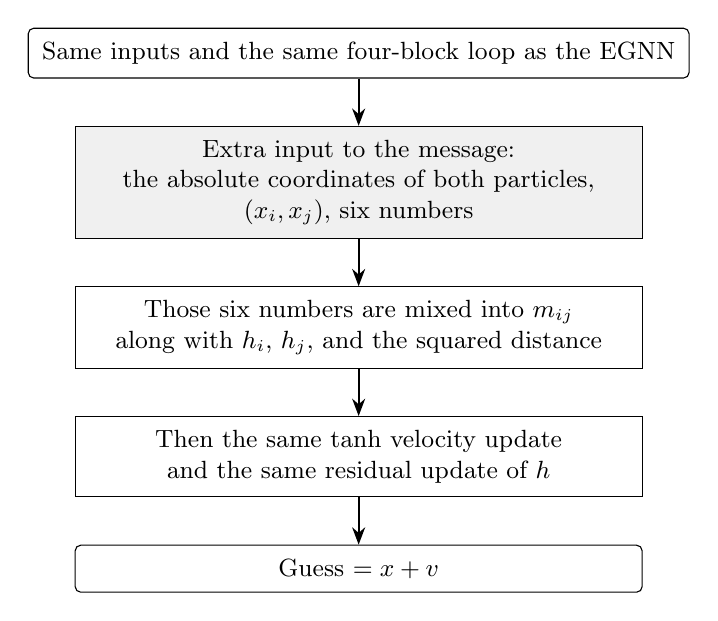
\begin{tikzpicture}
  \node[io] (in) {Same inputs and the same four-block loop as the EGNN};
  \node[diff, below=6mm of in] (abs) {Extra input to the message:\\the absolute coordinates of both particles,\\$(x_i, x_j)$, six numbers};
  \node[stage, below=6mm of abs] (msg) {Those six numbers are mixed into $m_{ij}$\\along with $h_i$, $h_j$, and the squared distance};
  \node[stage, below=6mm of msg] (rest) {Then the same tanh velocity update\\and the same residual update of $h$};
  \node[io, below=6mm of rest] (out) {Guess $= x + v$};
  \draw[arr] (in) -- (abs);
  \draw[arr] (abs) -- (msg);
  \draw[arr] (msg) -- (rest);
  \draw[arr] (rest) -- (out);
\end{tikzpicture}
\caption{Non-equivariant GNN.
The shaded box is the only change.
Because the message can see where the particles sit in the coordinate frame, a rotation of the input no longer rotates the output in the same way.}
\label{fig:noneq}
\end{figure}

\begin{figure}[ht]
\centering
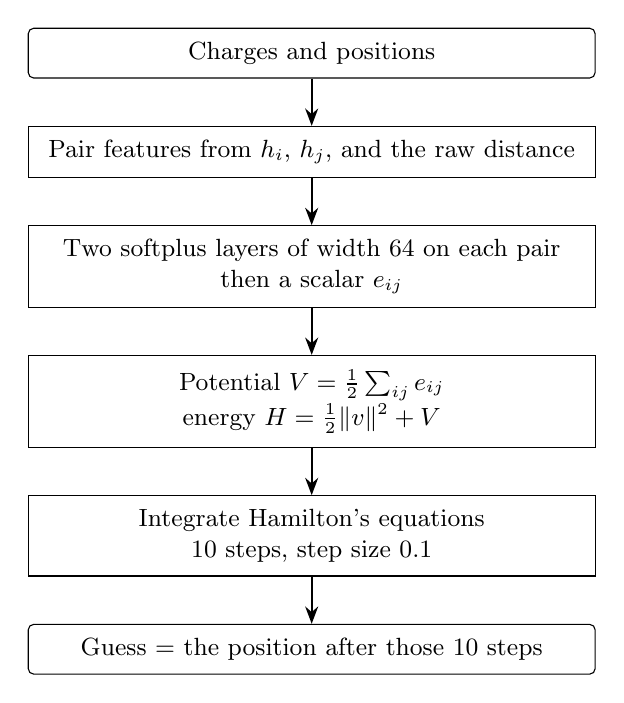
\begin{tikzpicture}
  \node[io] (in) {Charges and positions};
  \node[stage, below=6mm of in] (pair) {Pair features from $h_i$, $h_j$, and the raw distance};
  \node[stage, below=6mm of pair] (mlp) {Two softplus layers of width 64 on each pair\\then a scalar $e_{ij}$};
  \node[stage, below=6mm of mlp] (pot) {Potential $V = \tfrac12 \sum_{ij} e_{ij}$\\energy $H = \tfrac12 \|v\|^2 + V$};
  \node[stage, below=6mm of pot] (int) {Integrate Hamilton's equations\\10 steps, step size $0.1$};
  \node[io, below=6mm of int] (out) {Guess $= $ the position after those 10 steps};
  \draw[arr] (in) -- (pair);
  \draw[arr] (pair) -- (mlp);
  \draw[arr] (mlp) -- (pot);
  \draw[arr] (pot) -- (int);
  \draw[arr] (int) -- (out);
\end{tikzpicture}
\caption{Hamiltonian network.
The learned object is a scalar potential, not a direct position guess.
Block~1 and block~2 in its probe table are the two softplus layers of this potential, evaluated at the initial positions.
The net-force cosine compares $-\partial H/\partial x$ at the start with the true net Coulomb force.}
\label{fig:hnn}
\end{figure}

\begin{figure}[ht]
\centering
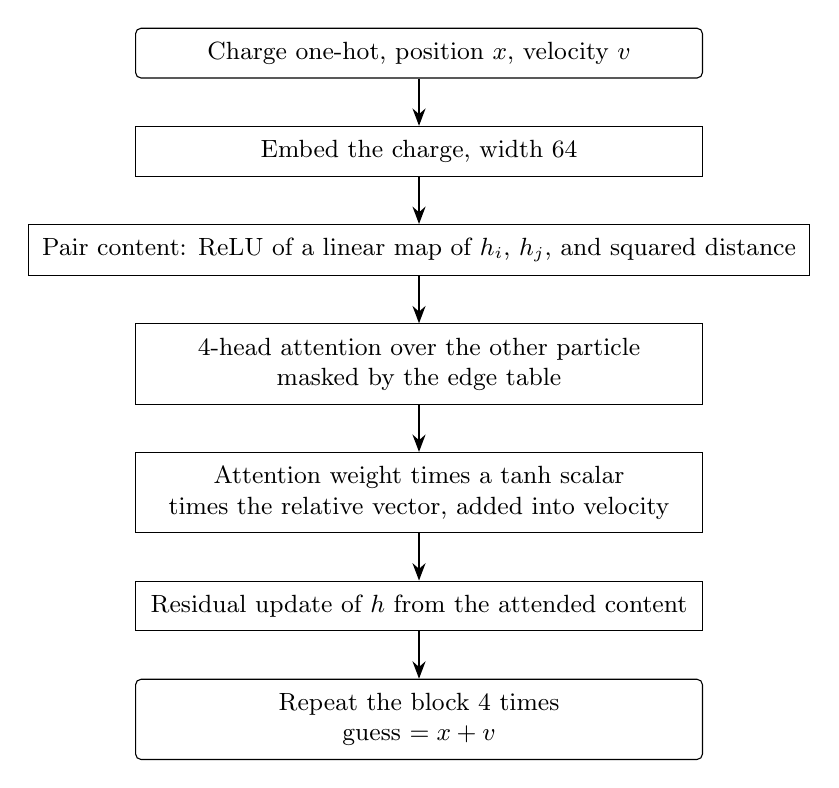
\begin{tikzpicture}
  \node[io] (in) {Charge one-hot, position $x$, velocity $v$};
  \node[stage, below=6mm of in] (emb) {Embed the charge, width 64};
  \node[stage, below=6mm of emb] (content) {Pair content: ReLU of a linear map of $h_i$, $h_j$, and squared distance};
  \node[stage, below=6mm of content] (attn) {4-head attention over the other particle\\masked by the edge table};
  \node[stage, below=6mm of attn] (vel) {Attention weight times a $\tanh$ scalar\\times the relative vector, added into velocity};
  \node[stage, below=6mm of vel] (hup) {Residual update of $h$ from the attended content};
  \node[io, below=6mm of hup] (out) {Repeat the block 4 times\\guess $= x + v$};
  \draw[arr] (in) -- (emb);
  \draw[arr] (emb) -- (content);
  \draw[arr] (content) -- (attn);
  \draw[arr] (attn) -- (vel);
  \draw[arr] (vel) -- (hup);
  \draw[arr] (hup) -- (out);
\end{tikzpicture}
\caption{Equivariant transformer.
This is not an Equiformer with irreducible representations.
The features that attention mixes are invariant scalars.
The arrow of the update still comes from the relative vector, scaled by those scalars.}
\label{fig:eqt}
\end{figure}

\section{Position error through training}

Each network was trained for 100 epochs on 2{,}400 systems and scored on 4{,}000 held-out systems.
The number is the mean squared error of the final $x,y,z$.
The logged epochs are 1, 20, 40, 60, 80, and 100.

\begin{table}[ht]
\centering
\caption{Validation position error.
Attention EGNN is the most accurate.
The Hamiltonian network's error rises after epoch~1.}
\label{tab:mse}
\begin{tabular}{lrrrrrr}
\toprule
Network & 1 & 20 & 40 & 60 & 80 & 100 \\
\midrule
Attention EGNN & 0.669 & 0.029 & 0.021 & 0.018 & 0.016 & 0.014 \\
Equivariant transformer & 0.242 & 0.128 & 0.087 & 0.091 & 0.086 & 0.051 \\
Non-equivariant GNN & 0.741 & 0.101 & 0.083 & 0.081 & 0.080 & 0.079 \\
EGNN & 0.127 & 0.093 & 0.092 & 0.090 & 0.090 & 0.090 \\
Hamiltonian network & 0.083 & 0.101 & 0.113 & 0.121 & 0.117 & 0.126 \\
\bottomrule
\end{tabular}
\end{table}

\section{Probe scores, block by block}

The probe freezes the trained network, runs the validation systems through it, and fits a separate straight line from each layer onto one fact.
Distance, charge product, and force magnitude are read from the pair message, one line for the 45 unordered pairs.
Charge is read from the per-particle vector $h$.
Potential energy is read from the average of the pair messages, one number per system.
Force direction is the cosine defined above, not an $R^2$.
Embed is the charge embedding before any block.
Pair facts are not probed there, because the pair message does not exist yet.
A blank cell means that measurement was not taken.

The line is fit on the training systems only.
The number in the table is the validation $R^2$, except the force rows, which are cosines.

\begin{table}[ht]
\centering
\caption{EGNN.
Distance, charge product, force magnitude, and potential energy are strongest in block~1.
Charge product and force magnitude fade in later blocks.
The force arrow stays near cosine $0$.}
\label{tab:egnn}
\begin{tabular}{lrrrrr}
\probehdr
Charge & 1.000 & 1.000 & 1.000 & 1.000 & 1.000 \\
Distance & & 0.999 & 0.982 & 0.957 & 0.800 \\
Charge product & & 0.997 & 0.362 & 0.432 & 0.132 \\
Force magnitude & & 0.951 & 0.561 & 0.468 & 0.345 \\
Potential energy & & 0.982 & 0.897 & 0.820 & 0.734 \\
Force direction & & 0.017 & $-0.004$ & 0.004 & 0.004 \\
\bottomrule
\end{tabular}
\end{table}

\begin{table}[ht]
\centering
\caption{Attention EGNN.
Charge is perfect in every layer.
Distance and charge product peak in the middle of the network and stay below the EGNN.
Potential energy is highest in block~2.
The force arrow rises only to $0.084$ by block~4.}
\label{tab:attn}
\begin{tabular}{lrrrrr}
\probehdr
Charge & 1.000 & 1.000 & 1.000 & 1.000 & 1.000 \\
Distance & & 0.397 & 0.741 & 0.759 & 0.502 \\
Charge product & & 0.273 & 0.480 & 0.509 & 0.257 \\
Force magnitude & & 0.813 & 0.645 & 0.706 & 0.788 \\
Potential energy & & 0.588 & 0.761 & 0.700 & 0.742 \\
Force direction & & 0.021 & 0.026 & 0.045 & 0.084 \\
\bottomrule
\end{tabular}
\end{table}

\begin{table}[ht]
\centering
\caption{Non-equivariant GNN.
Block~1 looks like the EGNN.
Charge product has collapsed by block~4.
Potential energy in block~4 is negative: the line is much worse than guessing the average.
The force arrow stays near $0$.}
\label{tab:noneq}
\begin{tabular}{lrrrrr}
\probehdr
Charge & 1.000 & 1.000 & 1.000 & 0.989 & 0.981 \\
Distance & & 0.993 & 0.968 & 0.944 & 0.695 \\
Charge product & & 0.915 & 0.233 & 0.091 & 0.003 \\
Force magnitude & & 0.860 & 0.400 & 0.393 & 0.240 \\
Potential energy & & 0.896 & 0.732 & 0.632 & $-2.344$ \\
Force direction & & 0.018 & $-0.004$ & 0.004 & $-0.004$ \\
\bottomrule
\end{tabular}
\end{table}

\begin{table}[ht]
\centering
\caption{Equivariant transformer.
Distance stays near $0.94$ in every block.
Charge product does not appear.
Force magnitude stays near $0.3$, and potential energy only reaches $0.36$ in block~4.
The force arrow is strongest in block~1, at cosine $0.129$, and fades.}
\label{tab:eqt}
\begin{tabular}{lrrrrr}
\probehdr
Charge & 1.000 & 1.000 & 1.000 & 1.000 & 1.000 \\
Distance & & 0.937 & 0.938 & 0.941 & 0.943 \\
Charge product & & 0.000 & 0.005 & 0.020 & 0.040 \\
Force magnitude & & 0.264 & 0.267 & 0.274 & 0.304 \\
Potential energy & & 0.000 & 0.034 & 0.092 & 0.360 \\
Force direction & & 0.129 & 0.096 & 0.076 & 0.041 \\
\bottomrule
\end{tabular}
\end{table}

\begin{table}[ht]
\centering
\caption{Hamiltonian network.
There is no block~3 or block~4.
Block~1 and block~2 are the two layers of the learned potential, at the initial positions.
Charge product, force magnitude, and potential energy appear in block~2.
The net-force row is a cosine, not an $R^2$.}
\label{tab:hnn}
\begin{tabular}{lrrr}
\toprule
Fact & Embed & Block 1 & Block 2 \\
\midrule
Charge & 1.000 & & \\
Distance & & 1.000 & 1.000 \\
Charge product & & 0.012 & 1.000 \\
Force magnitude & & 0.650 & 0.938 \\
Potential energy & & 0.056 & 0.887 \\
Net force & & & 0.085 \\
\bottomrule
\end{tabular}
\end{table}

\section{Deleting a high-scoring line}

A line was removed only when its validation $R^2$ was at least $0.8$.
Force-direction rows were not removed, because they are not fitted lines.
Removal means the component of the layer vector along that line is subtracted, and the same validation systems are run again.
The position error is measured before and after.
If the error rises, the guess was depending on that direction.
If the error stays put, the fact was readable and this particular line was not needed for the guess.

Many removals with $R^2 \ge 0.8$ left the error unchanged to three digits.
Table~\ref{tab:ablate} keeps the removals that moved the validation error by at least $0.005$.

\begin{table}[ht]
\centering
\caption{Deletions that changed the position error.
The largest change is force magnitude in block~1 of the non-equivariant network.}
\label{tab:ablate}
\begin{tabular}{llrr}
\toprule
Network & Line removed & Before & After \\
\midrule
Non-equivariant GNN & Force magnitude, block 1 & 0.079 & 0.458 \\
Hamiltonian network & Distance, block 2 & 0.126 & 0.323 \\
Equivariant transformer & Distance, block 1 & 0.051 & 0.216 \\
Non-equivariant GNN & Distance, block 1 & 0.079 & 0.114 \\
Non-equivariant GNN & Charge product, block 1 & 0.079 & 0.102 \\
Attention EGNN & Charge, block 2 & 0.014 & 0.028 \\
EGNN & Charge product, block 1 & 0.090 & 0.103 \\
Hamiltonian network & Distance, block 1 & 0.126 & 0.137 \\
Attention EGNN & Charge, embedding & 0.014 & 0.019 \\
Hamiltonian network & Charge, embedding & 0.126 & 0.120 \\
\bottomrule
\end{tabular}
\end{table}

The last row moves the wrong way by a small amount: the error goes down.
That is still a change, but it is not evidence that the network needed the deleted line.
The EGNN's perfect charge and distance scores are not in this table.
Deleting those lines left the position error at $0.090$.

\section{Assignment 2}

The assignment trained the same Coulomb task and reported validation error in the notebook discussion.
Three of those runs correspond to networks here.
The Hamiltonian network and the equivariant transformer were not in the assignment.

\begin{table}[ht]
\centering
\caption{Assignment~2 validation error next to the epoch-100 error of the closest network in this project.}
\label{tab:a2}
\begin{tabular}{llrr}
\toprule
Assignment 2 run & Network here & Assignment 2 & Here \\
\midrule
Attention & Attention EGNN & 0.0103 & 0.014 \\
Full EGNN & EGNN & 0.0945 & 0.090 \\
No equivariance & Non-equivariant GNN & 0.0579 & 0.079 \\
No residual & --- & 0.0896 & --- \\
No velocity & --- & 0.0983 & --- \\
No distance & --- & 0.1279 & --- \\
No tanh & --- & 11.46 & --- \\
\bottomrule
\end{tabular}
\end{table}

\end{document}
